\chapter{Data Warehouse Design}

\section{Choice of schema type}
Based on the available sources (market snapshots + reference JSON files described in the previous chapter), we selected a \textbf{constellation schema} (multiple fact tables sharing common dimensions). 
This design supports different analytical perspectives (transactions, attributes, undervalued detection) while reusing core dimensions such as \texttt{dim\_item} and \texttt{dim\_time}.

\section{Multidimensional model diagram}
\begin{figure}[H]
    \centering
    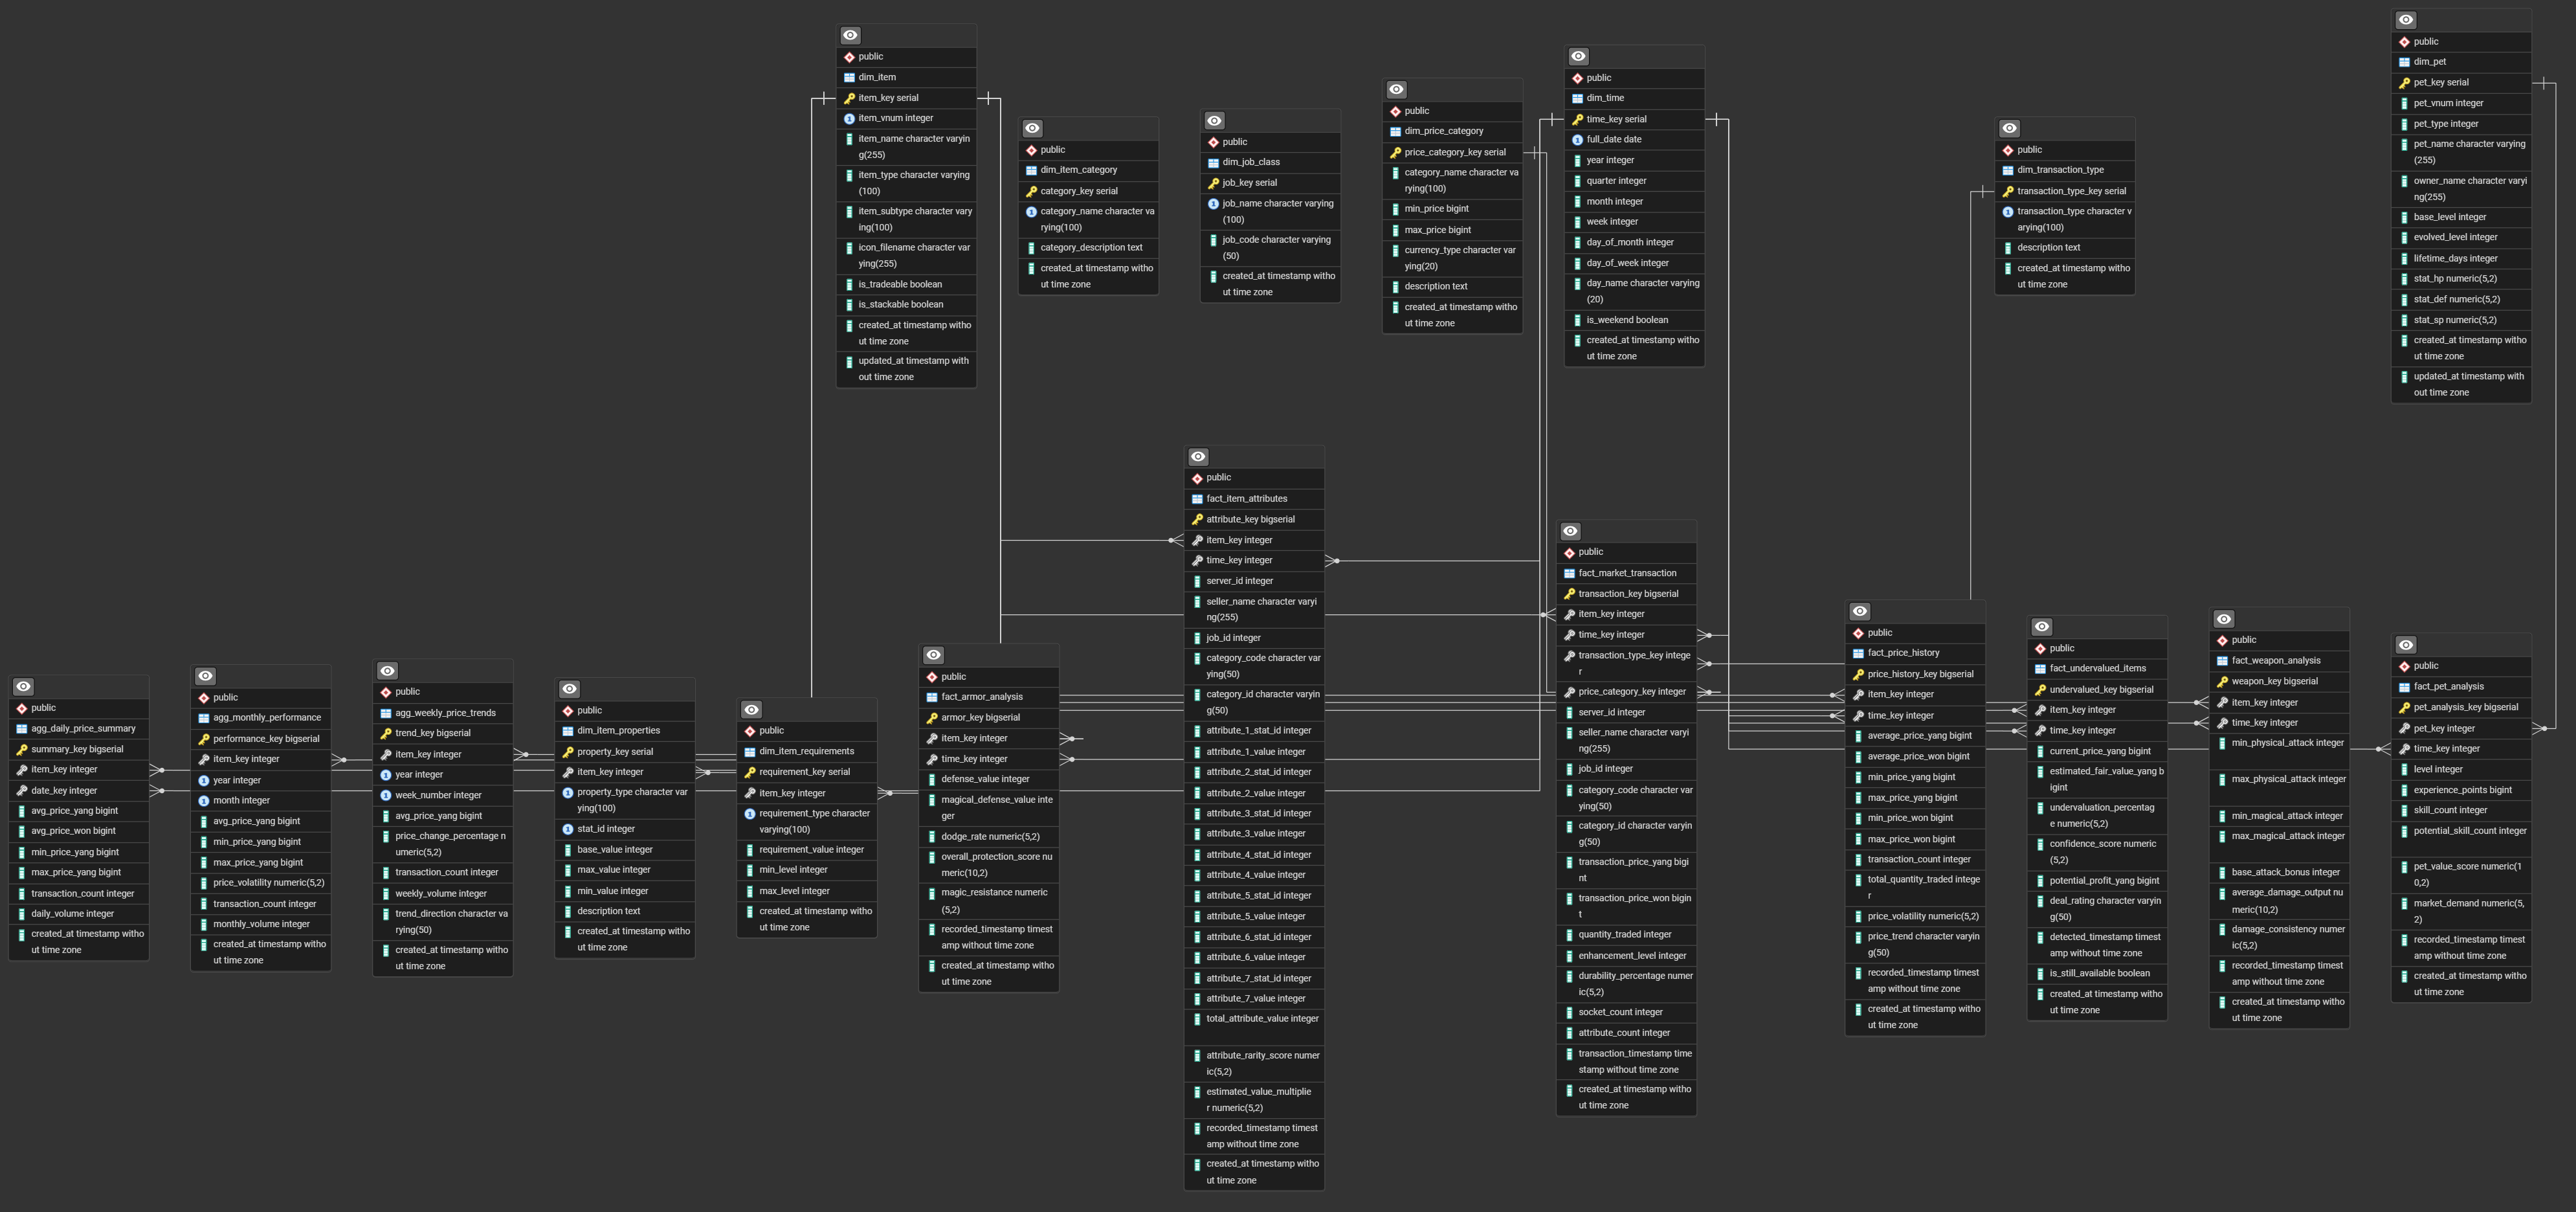
\includegraphics[width=0.92\linewidth]{Schema.png}
    \caption{Constellation schema overview (core tables used for analysis).}
    \label{fig:json-relationships}
\end{figure}


\section{Description of fact tables and dimensions}
\subsection{Core dimensions}
\begin{table}[!ht]
\centering
\caption{Main dimensions (excerpt)}
\begin{tabularx}{\linewidth}{@{}lX@{}}
\toprule
\textbf{Dimension} & \textbf{Role in analysis} \\
\midrule
\texttt{dim\_item} & Item reference: vnum, English name, type/subtype, tradeable/stackable flags. \\
\texttt{dim\_time} & Time axis for trends, daily/weekly/monthly aggregations. \\
\texttt{dim\_transaction\_type} & Separates listing/transaction semantics (when applicable). \\
\texttt{dim\_price\_category} & Enables bucketed analysis by price range. \\
\bottomrule
\end{tabularx}
\end{table}

\subsection{Main facts}
\begin{table}[!ht]
\centering
\caption{Main fact tables (excerpt)}
\begin{tabularx}{\linewidth}{@{}lX@{}}
\toprule
\textbf{Fact} & \textbf{Measures / KPIs} \\
\midrule
\texttt{fact\_market\_transaction} & transaction\_price\_yang/won, quantity, enhancement\_level; listing context (server, seller, category). \\
\texttt{fact\_item\_attributes} & up to 7 attribute stat/value pairs; rarity score; estimated value multiplier. \\
\texttt{fact\_price\_history} & average/min/max prices per day; volatility; trend direction. \\
\texttt{fact\_undervalued\_items} & undervaluation\%, confidence score, potential profit, deal rating. \\
\bottomrule
\end{tabularx}
\end{table}

\placeholderfigure{Full Multidimensional Model Diagram (detailed)}{0.92\linewidth}{6cm}

